%===========================================================
\chapter{Introduction}
%===========================================================

\section{What Vikasa is}
Vikasa (Sanskrit for ``development'' or ``unfolding'') is a \textbf{deterministic,
individual-based evolution simulator}. Every animal in its world inherits a body
genome and a behavioural temperament, perceives its surroundings, and decides for
itself what to do next. Populations forage, court, fight, raise young, starve,
age and evolve over generations. Nothing on screen is scripted: every birth,
death and clash is the outcome of explicit, inspectable rules evaluated by one
seeded random-number generator.

On top of that core, Vikasa asks a concrete real-world question:

\begin{quote}
\emph{Climate change is not only about how hot it gets, but whether life can adapt
in time. Fast breeders can evolve; slow breeders fall behind. Where is the line?}
\end{quote}

To answer it, Vikasa forces its world with real temperature records (NASA POWER
monthly reanalysis for Indian regions) and IPCC AR6 warming pathways, gives every
animal a heritable thermal optimum, and measures the \emph{critical rate} of
warming beyond which evolution can no longer keep a population alive. The answer,
$0.262\,^{\circ}$C per generation with inheritance against $0.067\,^{\circ}$C per
generation without, is then turned into two practical tools: the \textbf{Species
Risk Checker} and the \textbf{Conservation Planner}.

\section{The project at a glance}

\begin{table}[htbp]
\centering
\caption{Vikasa 2.3 at a glance}
\begin{tabularx}{\textwidth}{lL}
\toprule
\textbf{The question} & Can a population evolve fast enough to survive warming, and how fast is too fast? \\
\textbf{The answer} & With heritable heat tolerance a population survives warming up to 0.262\,$^{\circ}$C per generation, about 4$\times$ more than without inheritance. Under SSP5-8.5, species with generations longer than about 6 years fall behind. \\
\textbf{The tool} & Species Risk Checker: pick a place, describe a species, choose a future, and get an instant estimate, a live simulation and a 3D replay. \\
\textbf{The plan} & Conservation Planner: give it a watchlist and get, per species, the year breeding fails, the heat-tolerance boost that would save it, climate refuges and a ranked action list. \\
\textbf{The showcase} & Demo mode: a presenter hub with a talk timer, one-click launches and a narrated 3D autopilot. \\
\bottomrule
\end{tabularx}
\end{table}

\section{Version history}
Vikasa evolved through clearly separated releases. Knowing which release produced
which evidence matters, because changed coefficients change trajectories even for
the same seed.

\begin{table}[htbp]
\centering
\caption{Release history}
\begin{tabularx}{\textwidth}{lL}
\toprule
Version & Main additions \\
\midrule
1.0--1.1 & Deterministic engine, six-gene genome, Pygame laboratory, headless CLI, checkpoints, first Godot client with Observatory charts and wildlife behaviour (drives, utilities, home ranges, care, fights, culture). \\
Research upgrade & Gompertz mortality, generational development tracking, exact birth-cohort Price decomposition, trait geometry (PCA) exports, optional spatial plant/water ecology, controlled seed-blocked experiment laboratory, opt-in diploid preview. \\
2.0 & \emph{Living Biome}: GPU-instanced 3D wildlife at a locked 60 FPS on integrated graphics, binary push stream, director camera, lenses, day/night, visible weather, procedural soundscape, adaptive quality. \\
2.1 & Climate rescue: NASA POWER data, IPCC AR6 pathways, heritable thermal optimum, critical-rate sweep, Sobol sensitivity, Gaussian-process surrogate, offline report. \\
2.2 & Species Risk Checker, Demo mode with presenter hub and 3D autopilot, one-app home screen and a single desktop shortcut. \\
2.3 & Conservation Planner: watchlist triage, breeding-failure years, assisted gene-flow sizing, refuge search, 14 new survey sites (24 total). \\
\bottomrule
\end{tabularx}
\end{table}

\section{Design principles}
Five principles recur across the code base and explain many design decisions
documented later.
\begin{enumerate}[leftmargin=*]
\item \textbf{The engine is authoritative.} One Python \code{SimulationEngine}
owns all state. Renderers, charts and web apps observe snapshots or issue explicit
commands; none decide outcomes.
\item \textbf{Determinism.} One NumPy PCG64 generator, stable integer IDs for
ordering and tie-breaking, and seeded schedules mean the same configuration and
seed reproduce the same world on the same platform.
\item \textbf{Honest evidence.} Extinct and failed runs are retained, uncertainty
is reported with intervals, missing data stays missing (never plotted as zero),
and pre-registered criteria that failed are published as failures.
\item \textbf{Inspectability.} Every animal exposes its current action, the
reason for it and the utility of each alternative. Every evidence package carries
configuration and source hashes and a SHA-256 manifest.
\item \textbf{Presentability.} The same science is delivered through a 3D
showcase that runs smoothly on an ordinary laptop, so non-specialists can see
what the numbers mean.
\end{enumerate}

\section{Code base size}
Vikasa 2.3 contains about 12{,}100 lines of Python in \code{src/} and 6{,}200 lines
of Python tests, about 5{,}700 lines of GDScript and GPU shader code in
\code{godot/}, and 554 collected automated tests (395 test functions, many of them
parametrised), plus nine headless Godot smoke and capture scripts.

%===========================================================
\chapter{Installation and Quick Start}
%===========================================================

\section{Requirements}
\begin{itemize}[leftmargin=*]
\item Python 3.12 or newer.
\item Runtime dependencies (installed automatically): NumPy $\ge$ 2.1, pandas
$\ge$ 2.2, Matplotlib $\ge$ 3.9, pygame-ce $\ge$ 2.5, scikit-learn $\ge$ 1.5, SciPy $\ge$ 1.14.
\item Development extras: pytest, pytest-cov, Hypothesis and Ruff
(\code{pip install -e .[dev]}).
\item Godot 4 for the 3D Living Biome, on a graphics-capable desktop
(Windows, macOS or Linux). No mobile build is provided.
\end{itemize}
The package is built with Hatchling and exposes one console entry point,
\code{vikasa = evolution\_sim.cli:main}.

\section{Windows}
\begin{lstlisting}
winget install --id GodotEngine.GodotEngine --exact --scope user
py -3.12 -m venv .venv
.\.venv\Scripts\python.exe -m pip install --upgrade pip
.\.venv\Scripts\python.exe -m pip install -e .
.\.venv\Scripts\vikasa.exe shortcut      # one "Vikasa" desktop shortcut
.\.venv\Scripts\vikasa.exe app           # open the Vikasa home screen
\end{lstlisting}
The launcher automatically detects a per-user WinGet Godot installation. If Godot
lives elsewhere, pass \code{--godot-path} or set the environment variable
\code{VIKASA\_GODOT\_BINARY}.

\section{macOS}
\begin{lstlisting}
brew install python@3.12
brew install --cask godot
python3.12 -m venv .venv
source .venv/bin/activate
python -m pip install --upgrade pip
python -m pip install -e .
vikasa godot --config config/showcase.json --seed 2026 \
  --godot-path /Applications/Godot.app/Contents/MacOS/Godot
\end{lstlisting}

\section{Linux (Ubuntu 24.04+)}
On Linux the bridge and the client run in two terminals.
\begin{lstlisting}
sudo apt update
sudo apt install -y python3.12 python3.12-venv flatpak
flatpak remote-add --user --if-not-exists flathub \
  https://flathub.org/repo/flathub.flatpakrepo
flatpak install --user -y flathub org.godotengine.Godot
python3.12 -m venv .venv && source .venv/bin/activate
python -m pip install -e .
# Terminal 1
vikasa serve --config config/showcase.json --seed 2026
# Terminal 2
flatpak run org.godotengine.Godot --path "$PWD/godot"
\end{lstlisting}

\section{The desktop shortcut}
\code{vikasa shortcut} writes a single \emph{Vikasa} shortcut that opens the home
screen through \code{pythonw.exe}, so no console window appears. Re-running it
replaces older Vikasa shortcuts, including ones that went straight into the 3D
biome. Optional direct shortcuts are available with \code{--only biome},
\code{--only demo} or \code{--only risk}; \code{--name} and \code{--desktop}
change the shortcut name and location.

\note{\textbf{Troubleshooting a shortcut that does nothing.} Run
\code{vikasa shortcut} from a normal terminal, not from inside a sandboxed agent.
A sandbox can hide the project files from Windows while the shortcut is saved, and
Windows then stores an empty target. Check the target with
\code{(New-Object -ComObject WScript.Shell).CreateShortcut(...).TargetPath}; it
must print the path to \code{.venv\textbackslash Scripts\textbackslash pythonw.exe}.}

\section{First run checklist}
\begin{enumerate}[leftmargin=*]
\item \code{vikasa validate --config config\textbackslash showcase.json} confirms the configuration parses.
\item \code{vikasa app} opens the home screen in the browser on \code{http://127.0.0.1:8787}.
\item Click \emph{Living Biome}. The bridge starts, Godot opens, and 64 founders appear.
\item Press \textbf{F1} in the 3D client for the field guide listing every shortcut.
\item Press \textbf{G} for the Observatory graphs and click any animal to see why it acts.
\end{enumerate}

%===========================================================
\chapter{Feature Tour}
%===========================================================

\section{The home screen}
\begin{figure}[htbp]
\centering
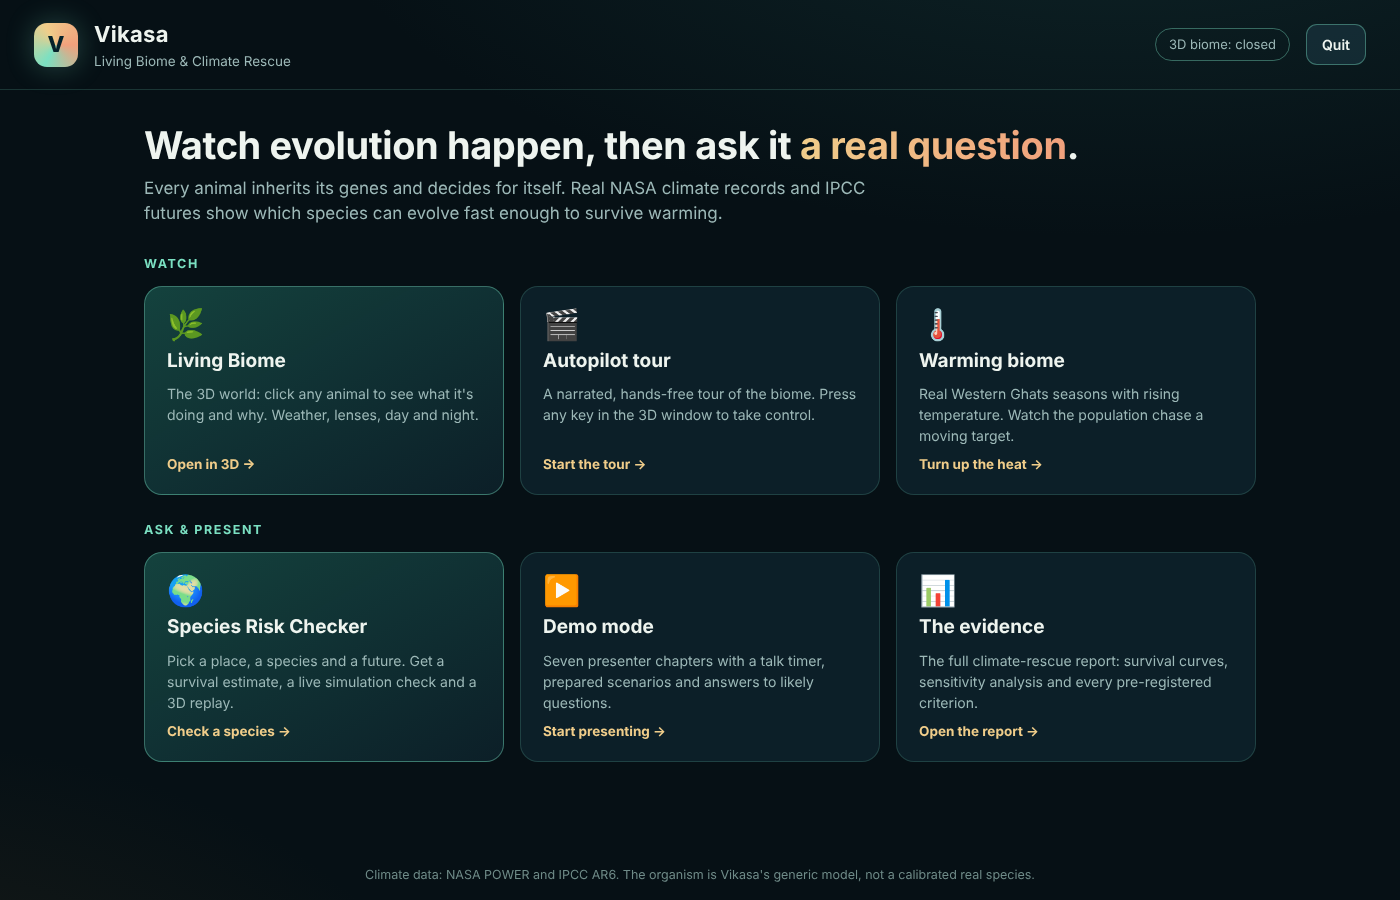
\includegraphics[width=0.85\textwidth]{vikasa-home.png}
\caption{The Vikasa home screen launches every feature with one click.}
\end{figure}
The home screen is served by the local application server on port 8787. It shows
whether a 3D window is open, can close it, and has a \emph{Quit} button that
shuts every Vikasa process down. Only one Vikasa runs per port; an older running
copy is replaced automatically.

\begin{table}[htbp]
\centering
\caption{Home-screen tiles}
\begin{tabularx}{\textwidth}{lL}
\toprule
Tile & What it opens \\
\midrule
Living Biome & The 3D world on the showcase configuration. \\
Autopilot tour & The narrated, hands-free 3D director's cut. \\
Warming biome & The 3D world with real Western Ghats seasons and rising temperature. \\
Species Risk Checker & The browser app for one place and one species (Chapter~\ref{ch:risk}). \\
Demo mode & The seven-chapter presenter hub. \\
The evidence & The committed climate-rescue report. \\
Conservation Planner & Watchlist to rescue plan (Chapter~\ref{ch:planner}). \\
\bottomrule
\end{tabularx}
\end{table}

\section{The Living Biome}
The 3D client renders the whole population with GPU instancing and lets the user
watch it like a nature film. Its main tools:
\begin{itemize}[leftmargin=*]
\item \textbf{Director (C)}: an autonomous camera that finds clashes, newborns,
alphas and families and captions them with letterbox lower-thirds. It only quotes
an explanation when it matches the action on screen.
\item \textbf{Lenses (V)}: recolour animals by coat, action, energy, dynasty
(maternal line), generation depth or temperament; the radar follows the lens.
\item \textbf{Daylight (N)}: cycle, day, golden hour and night, with eyeshine,
fireflies and glowing food after dark (presentation only).
\item \textbf{Legends (L)}: the living elder, most prolific parent, champion,
deepest descendant, best forager and largest dynasty; click to fly there.
\item \textbf{Photo (P)} and \textbf{F12} screenshots to \code{Pictures/Vikasa}.
\item \textbf{World tools (T)}: apply drought, heat, storm, wildfire, cold,
disease, a food-growth bloom, or click to scatter ten audited food patches.
\end{itemize}

\begin{figure}[htbp]
\centering
\begin{minipage}{0.49\textwidth}\centering
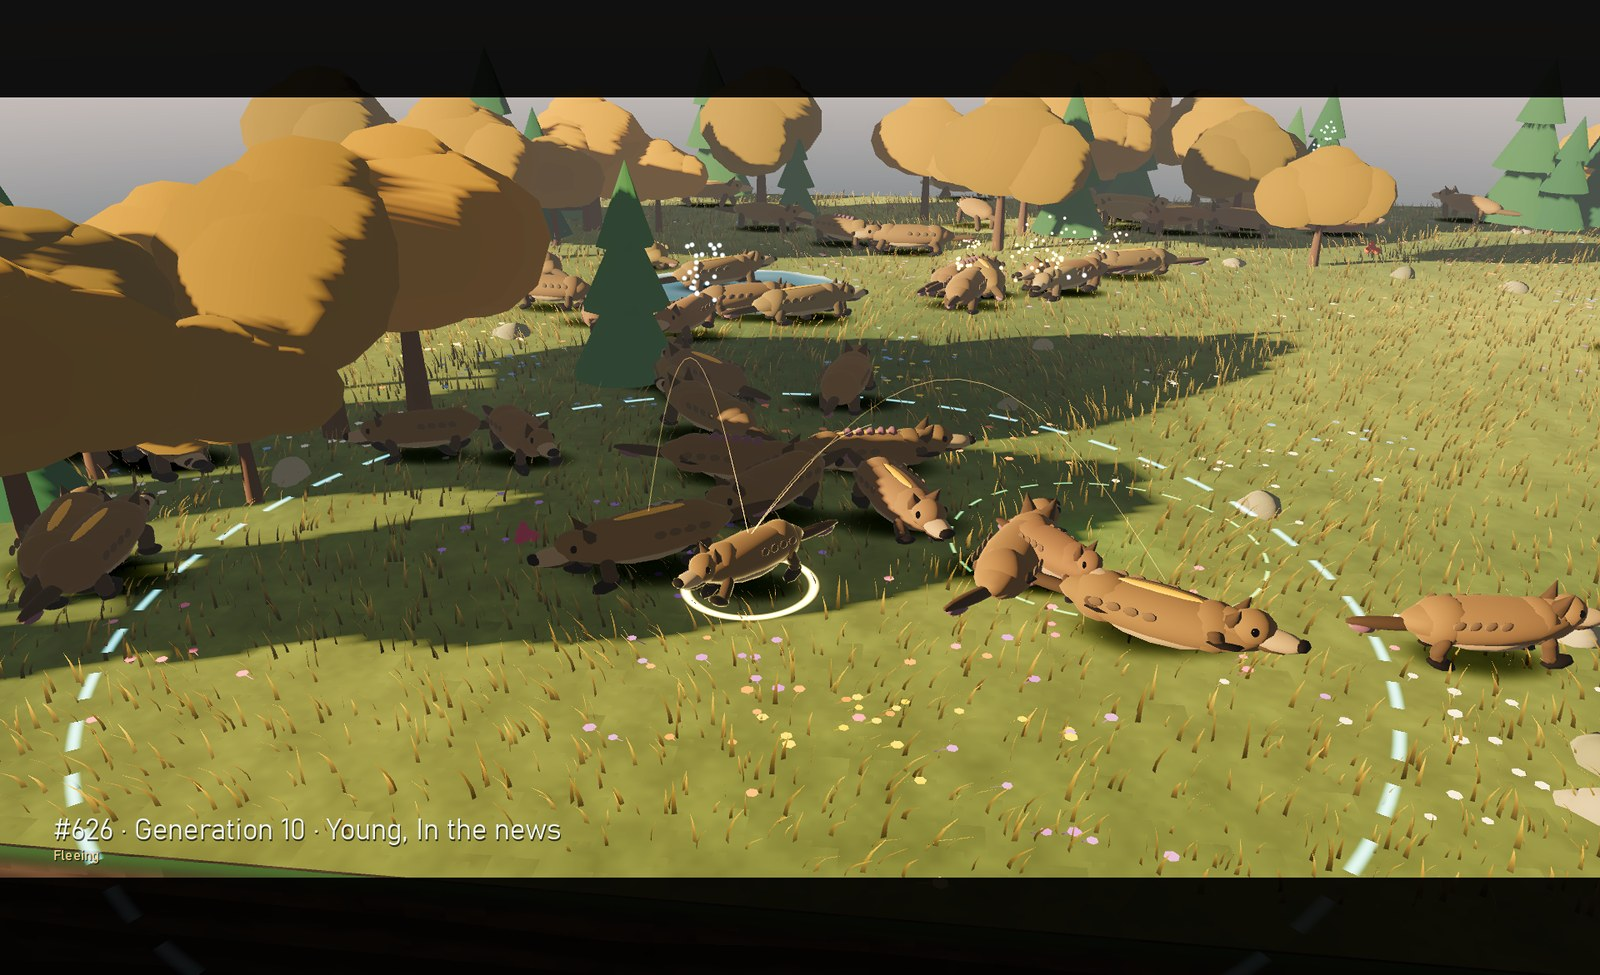
\includegraphics[width=\linewidth]{showcase-director.jpg}\\[-2pt]
{\small (a) Director's cut}
\end{minipage}\hfill
\begin{minipage}{0.49\textwidth}\centering
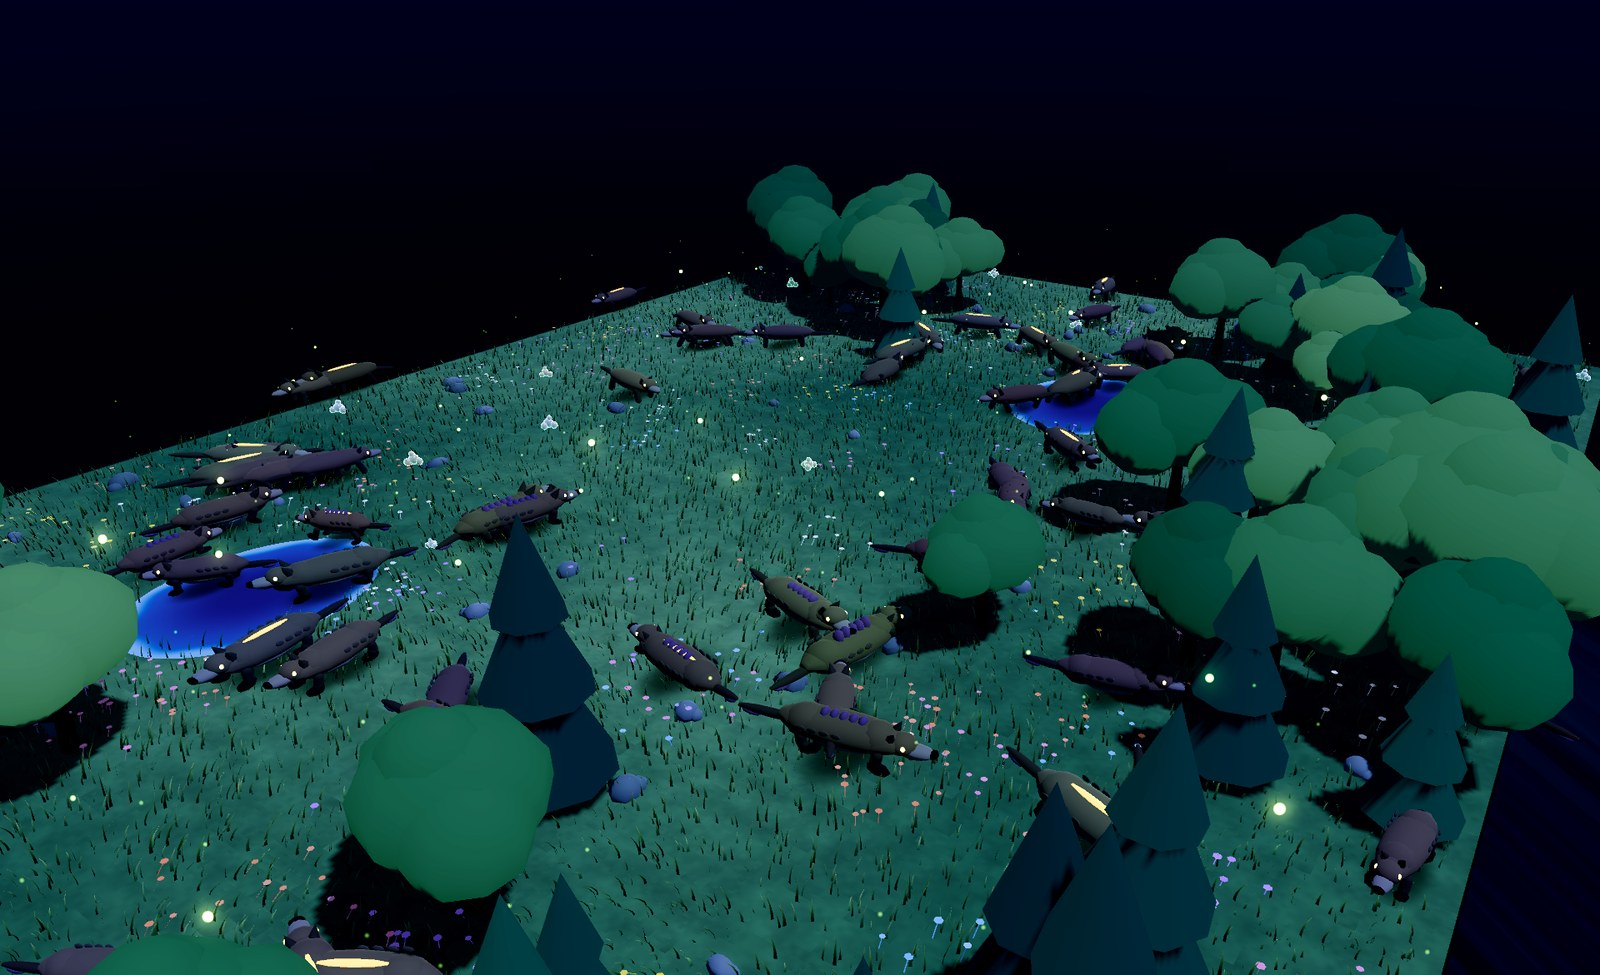
\includegraphics[width=\linewidth]{showcase-night.jpg}\\[-2pt]
{\small (b) Night with eyeshine and fireflies}
\end{minipage}\\[6pt]
\begin{minipage}{0.49\textwidth}\centering
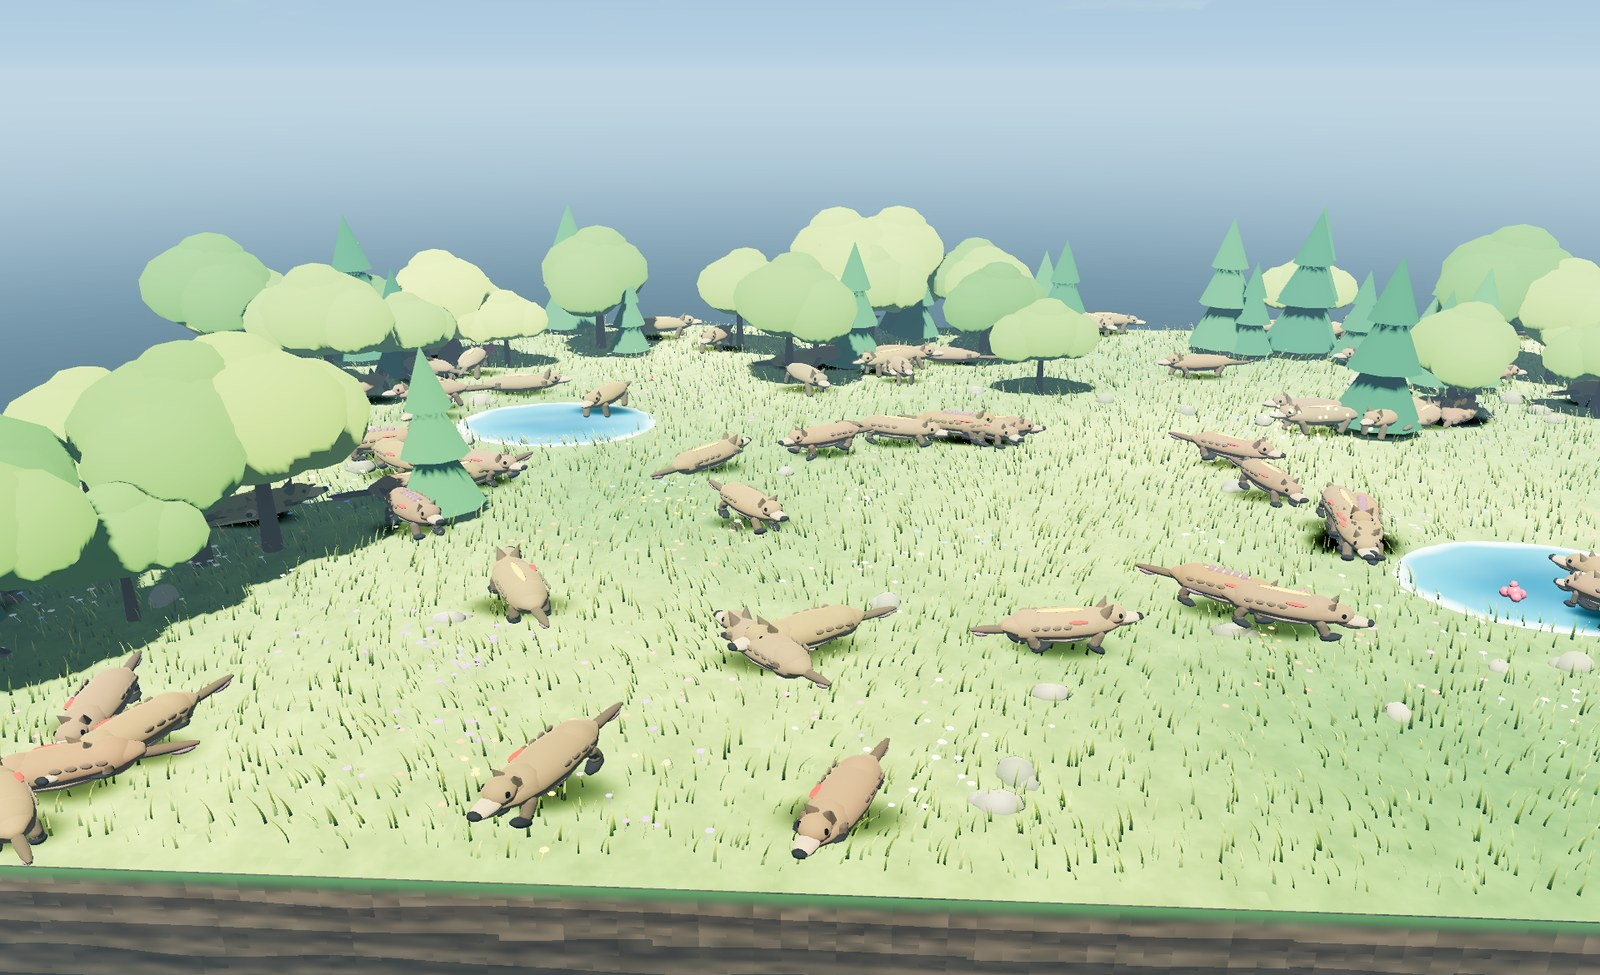
\includegraphics[width=\linewidth]{showcase-storm.jpg}\\[-2pt]
{\small (c) Visible storm}
\end{minipage}\hfill
\begin{minipage}{0.49\textwidth}\centering
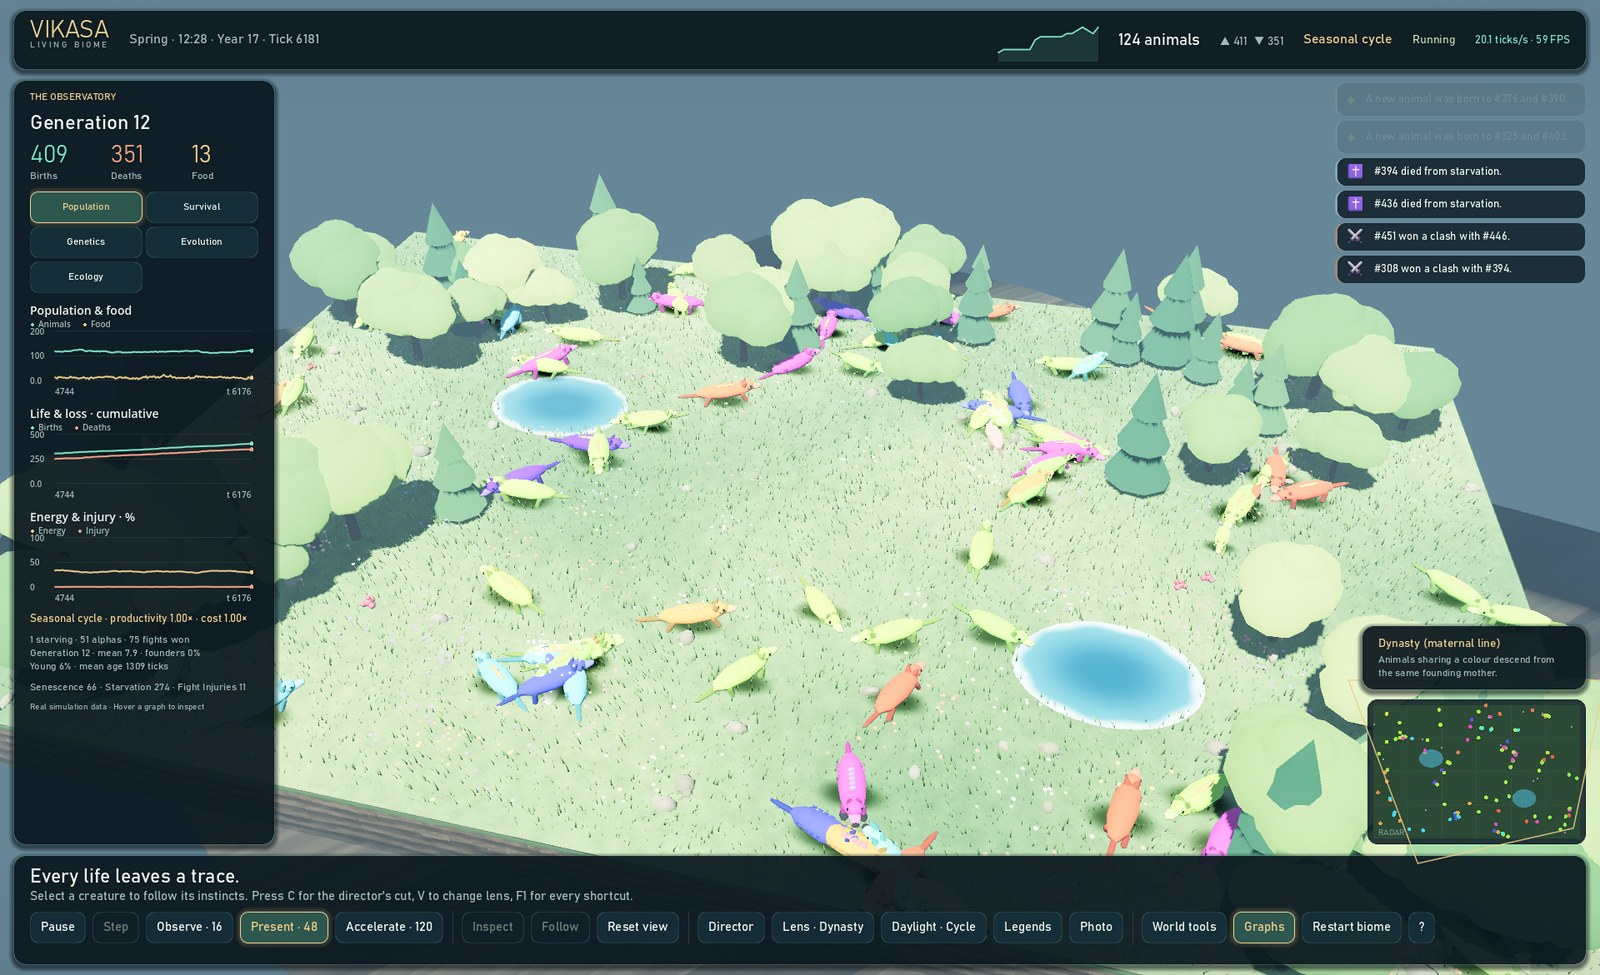
\includegraphics[width=\linewidth]{showcase-lens-dynasty.jpg}\\[-2pt]
{\small (d) Dynasty lens with radar}
\end{minipage}
\caption{Living Biome presentation modes. All captures are real seeded bridge states.}
\end{figure}

\begin{figure}[htbp]
\centering
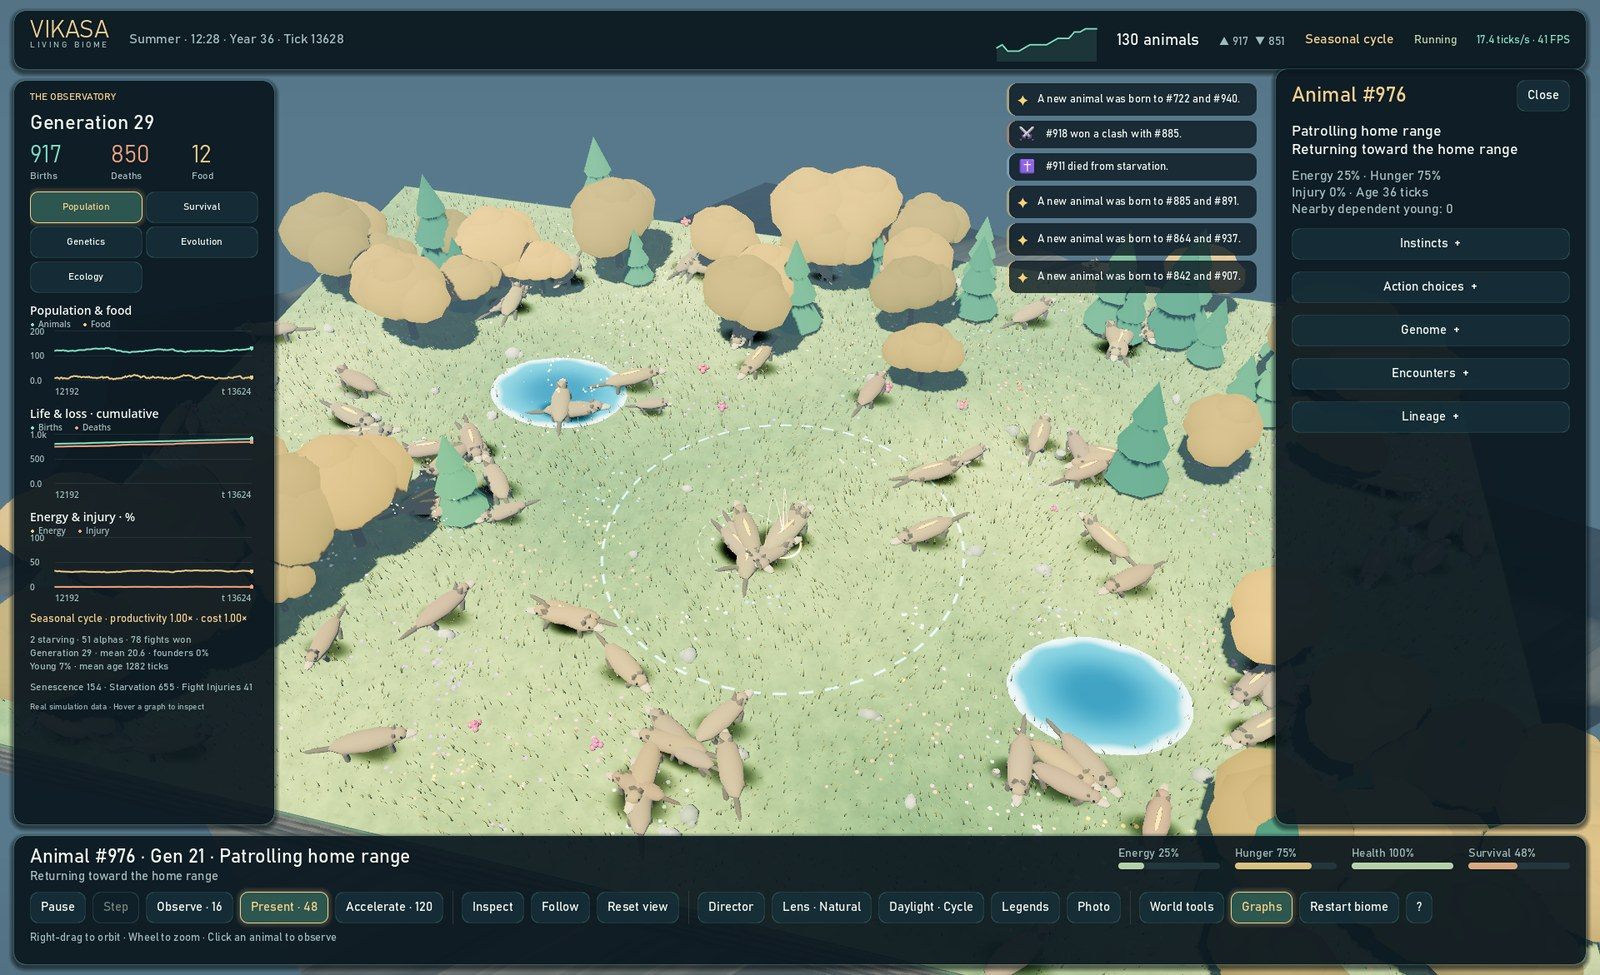
\includegraphics[width=0.95\textwidth]{showcase-interface.jpg}
\caption{Full interface: inspector, event feed, radar minimap and Observatory.}
\end{figure}

Clicking a creature opens its profile: current action and reason, energy, hunger,
injury, instincts (the six drives), top action choices with utilities, genes,
encounters, satisfaction and lineage. In the world, a halo, sensing radius, home
range, a line to the current target and threads to living parents and dependent
young appear (Fig.~\ref{fig:closeup}).

\begin{figure}[htbp]
\centering
\begin{minipage}{0.49\textwidth}\centering
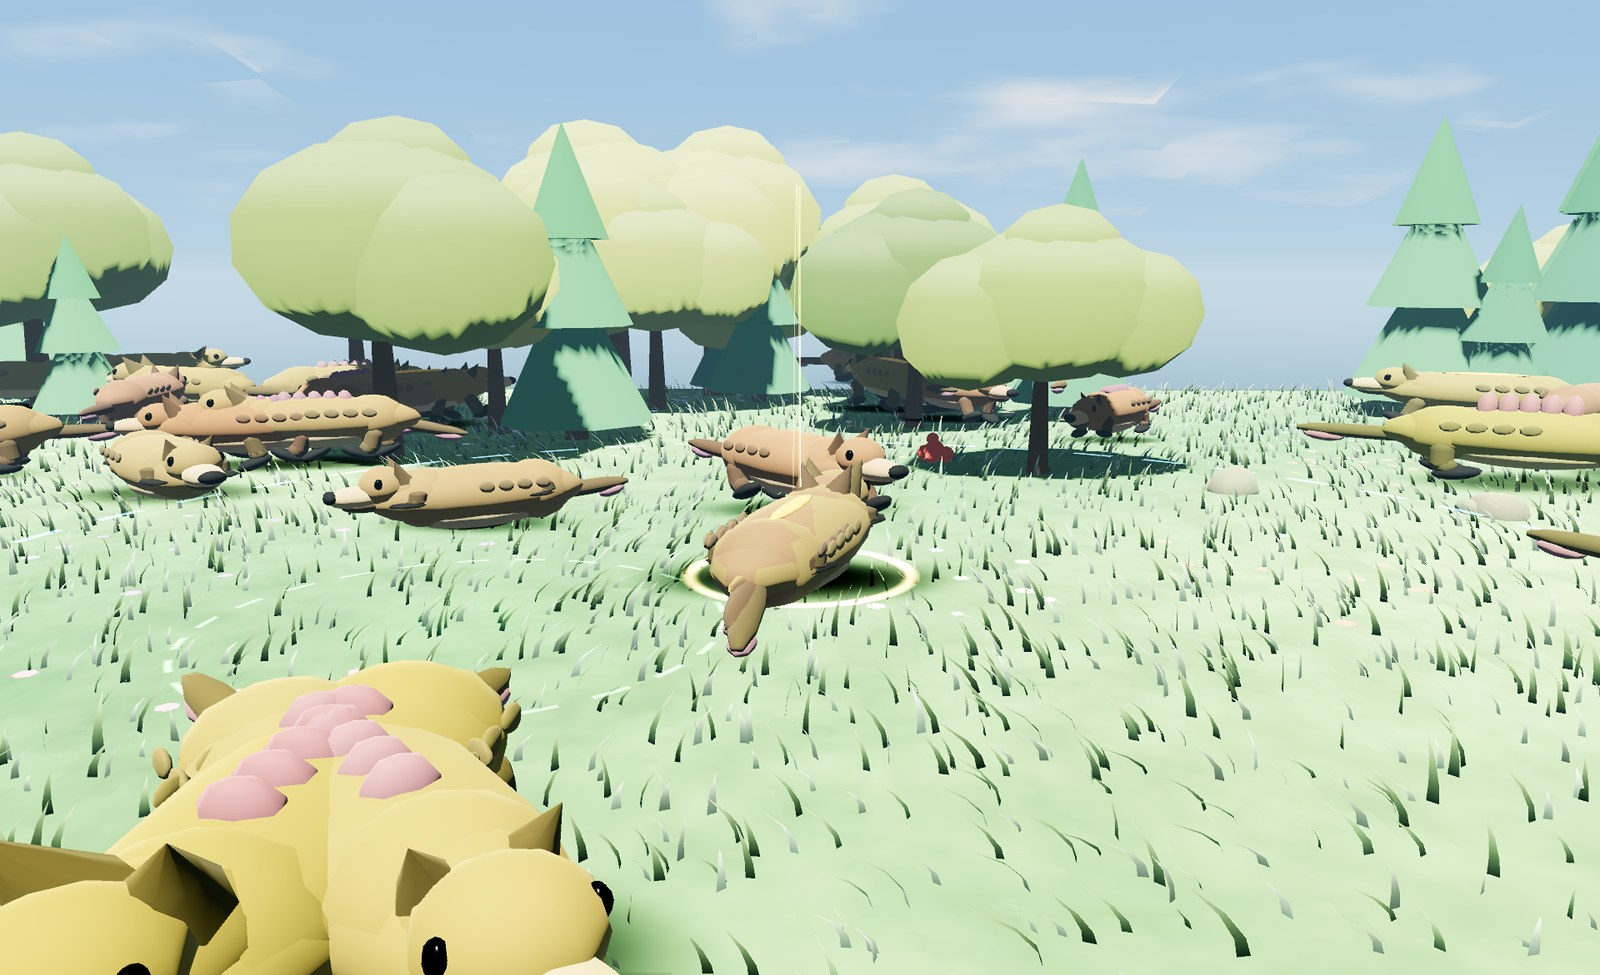
\includegraphics[width=\linewidth]{showcase-closeup.jpg}\\[-2pt]
{\small (a) Selection with kin threads}
\end{minipage}\hfill
\begin{minipage}{0.49\textwidth}\centering
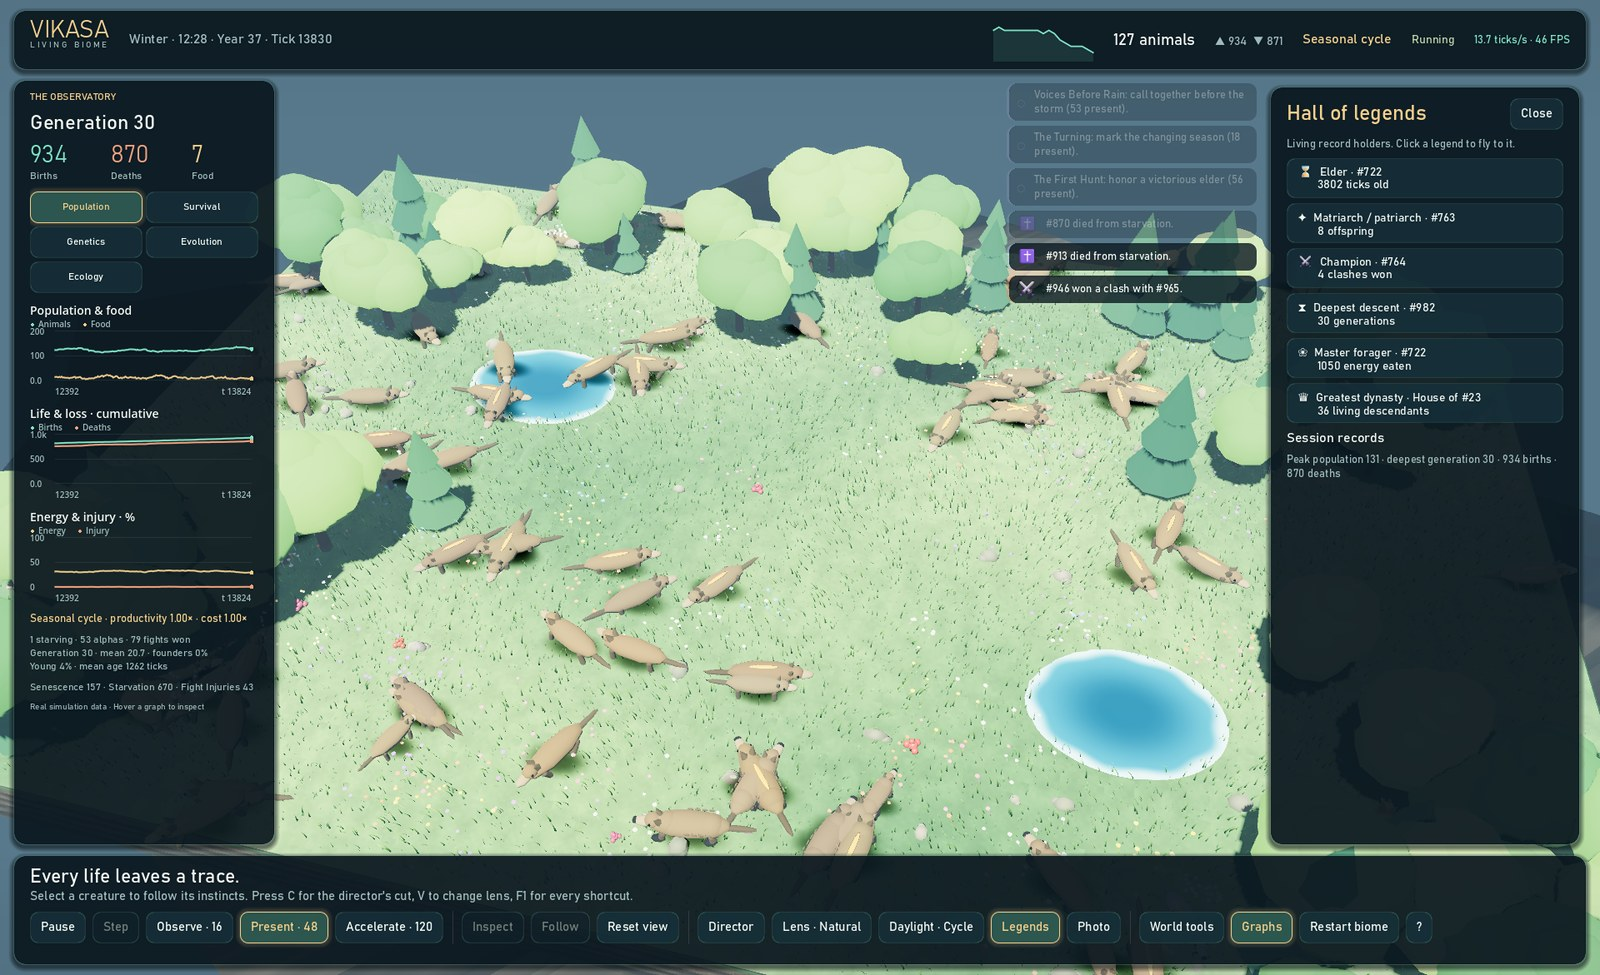
\includegraphics[width=\linewidth]{showcase-legends.jpg}\\[-2pt]
{\small (b) Hall of legends}
\end{minipage}
\caption{Inspecting individuals.}
\label{fig:closeup}
\end{figure}

\section{Species Risk Checker}
A browser application and a terminal command that, for any place and species,
return an instant estimate, an optional live simulation and a 3D replay. It is
documented fully in Chapter~\ref{ch:risk}.
\begin{lstlisting}
vikasa risk check --place hyderabad --generation-years 6 --ssp SSP5-8.5

Species Risk Checker - Hyderabad - SSP5-8.5
  Climate     mean 26.0 C, seasons +/-6.4 C (NASA POWER 1991-2020)
  Organism    generation 6 years, tolerance 9.6 C (local)
  Today       viable (peak hot season stress 0.55; breeding stops above 0.7)
  Warming     0.247 C per generation (94% of the critical rate)
  Danger line generations longer than 6.4 years fall behind under SSP5-8.5
  Survival    58% with evolution, 1% without
  VERDICT     AT RISK
\end{lstlisting}

\section{Conservation Planner}
Turns a CSV watchlist into a ranked rescue plan with breeding-failure years,
assisted gene-flow sizing, refuges and an action list; documented in
Chapter~\ref{ch:planner}.

\section{Demo mode}
\code{vikasa demo} opens a seven-chapter presenter hub (Table~\ref{tab:demo}).
Keys: $\leftarrow$/$\rightarrow$ move between chapters, Space starts the talk timer,
F toggles fullscreen and 1--7 jump directly. \code{--biome-only} opens just the 3D
autopilot.

\begin{table}[htbp]
\centering
\caption{Demo-mode chapters}
\label{tab:demo}
\begin{tabularx}{\textwidth}{clcL}
\toprule
\# & Chapter & Time & On screen \\
\midrule
1 & The question & 30 s & Headline results and the talk track \\
2 & The living biome & 90 s & One click opens the 3D biome on autopilot \\
3 & Warming in 3D & 60 s & Western Ghats seasons with rising temperature \\
4 & Species Risk Checker & 90 s & Prepared scenarios: frog in Hyderabad, six-year species, tortoise in Delhi \\
5 & The evidence & 45 s & Survival curve and all eight pre-registered criteria \\
6 & Under the hood & 45 s & Architecture and live statistics (tests, lines of code, frame rate) \\
7 & Judges' questions & --- & Prepared answers to the six most likely questions \\
\bottomrule
\end{tabularx}
\end{table}

The 3D autopilot (\code{godot/scripts/DemoPilot.gd}) runs a narrated four-minute
loop: director camera, dynasty and generation lenses, nightfall, a storm, a food
bloom and a fast-forward burst. Any key or click hands control back and restores
the user's settings. It is headless-tested by \code{godot/tests/DemoPilotSmoke.gd}.

\section{The Pygame laboratory}
\code{vikasa ui} opens the 2D laboratory with a launch configurator, presets,
organism selection, trait and lineage inspection, trails, perception overlays and
charts. Keys: Enter launches, Space pauses, 1--5 choose 1, 2, 4, 8 or 16 ticks per
rendered frame, R restarts with the same seed, C opens setup, P toggles perception,
T toggles trails, Ctrl+S saves a checkpoint, Ctrl+O loads it, E exports, and ? or
Escape opens help. Speed changes ticks per frame, never the equations.

\begin{figure}[htbp]
\centering
\begin{minipage}{0.49\textwidth}\centering
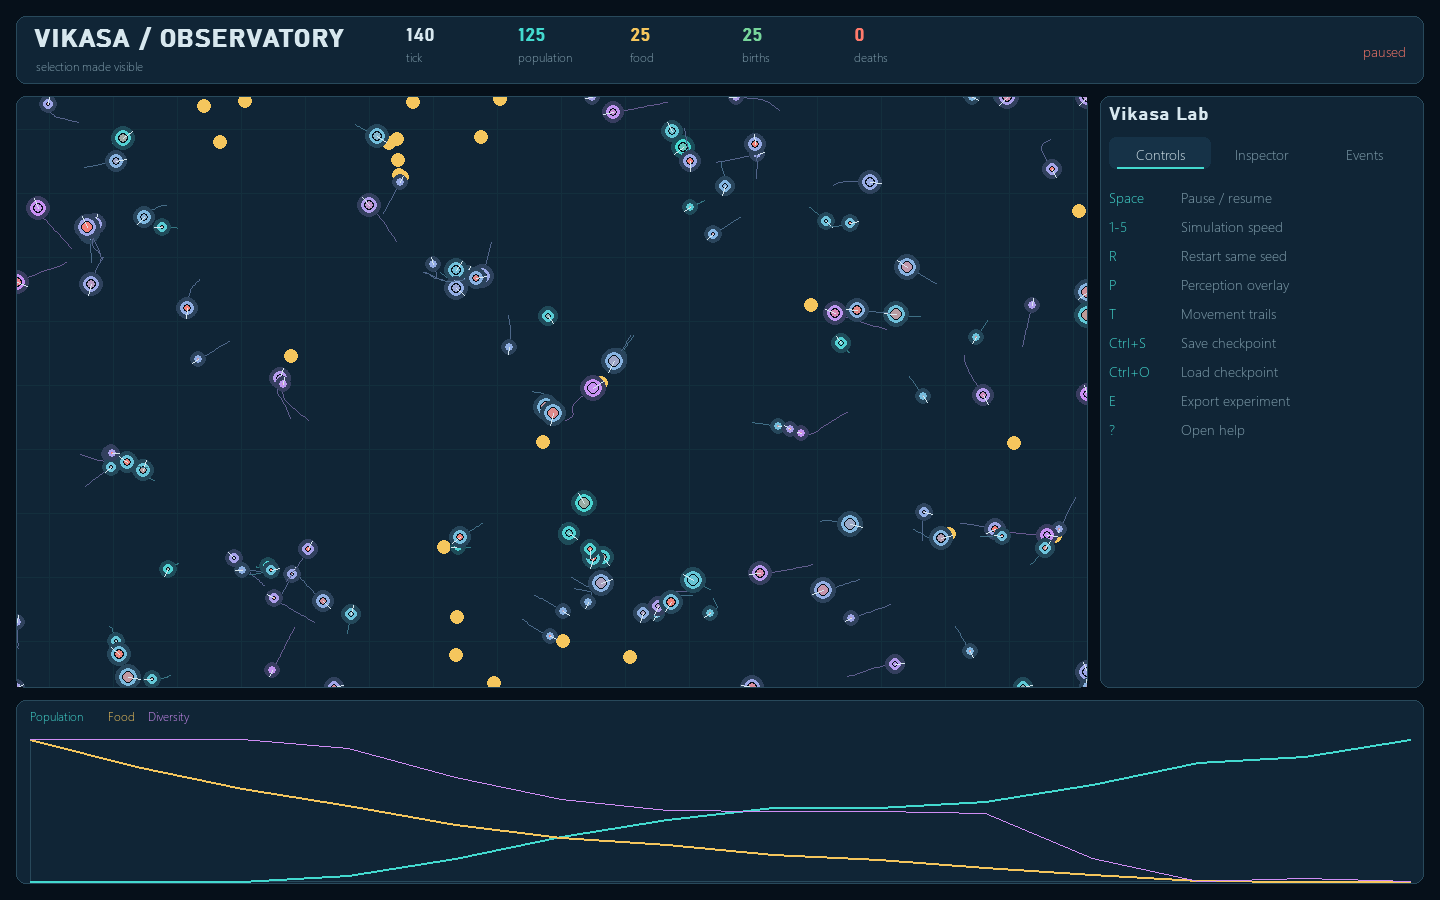
\includegraphics[width=\linewidth]{laboratory.png}\\[-2pt]
{\small (a) Laboratory view}
\end{minipage}\hfill
\begin{minipage}{0.49\textwidth}\centering
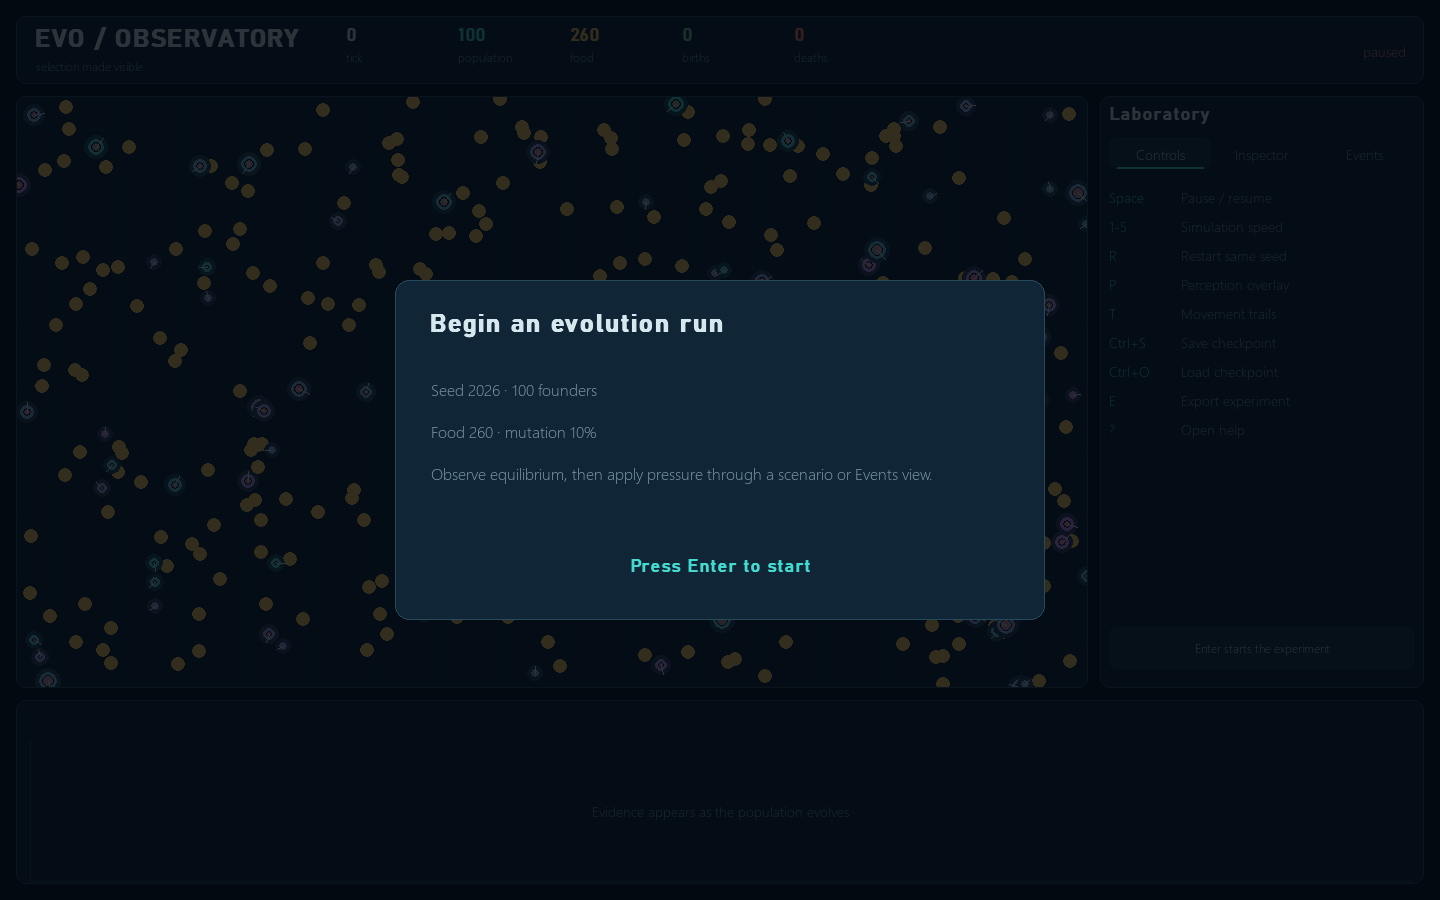
\includegraphics[width=\linewidth]{setup.png}\\[-2pt]
{\small (b) Launch configurator}
\end{minipage}
\caption{The Pygame 2D laboratory.}
\end{figure}
